\documentclass[12pt]{article}

\usepackage[utf8]{inputenc}
\usepackage[T1]{fontenc}
\usepackage[francais]{babel}
\usepackage{setspace}
\usepackage{graphicx}
\usepackage{ulem}
\usepackage{url}
\usepackage{multicol}
\usepackage[top=1cm,left=1cm,right=1cm,bottom=2cm]{geometry}

\usepackage{vwcol}
\usepackage[hidelinks]{hyperref}


\begin{document}

\begin{figure}
	\centering
	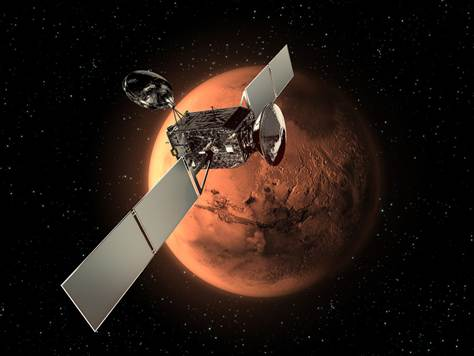
\includegraphics[scale=0.8]{images/logo.jpg}
\end{figure}

\hspace{\fill}

\begin{center}
	\LARGE{\textbf{Projet ExoLife}}
\end{center}


\begin{center}
\textbf{Analyse d'images pour but de trouver une source de vie dans l'univers, autre que sur Terre.}\\
\end{center}

\vspace{\fill}

\begin{flushright}
	\bsc{Chiaverini} Marie\\
	\bsc{Blochet} Tanguy\\
	\bsc{Saclier} Baptiste\\
\end{flushright}

\clearpage

\tableofcontents

\clearpage
\subsection{Sous-Mission A1}
\clearpage
	\subsection{Sous-mission A2}
	\begin{vwcol}[widths={0.65,0.2}, rule=0pt]
		\begin{minipage}{0.7\textwidth}
			\paragraph{Objectifs de la mission}

			Déterminer la quantité de méthane dans l'atmosphère de la planète Mars, afin de déterminer si il y a une présence de vie sur cette planète. Pour se faire nous avions à disposition une photographie satellite de la surface de Mars.
		\end{minipage}

		\begin{minipage}{0.3\textwidth}
			\begin{flushright}
				\paragraph{Technique utilisée}
			
				Proportion \&
				Moyenne
			\end{flushright}
		\end{minipage}
	\end{vwcol} 

	\begin{figure}[h]
		\centering
		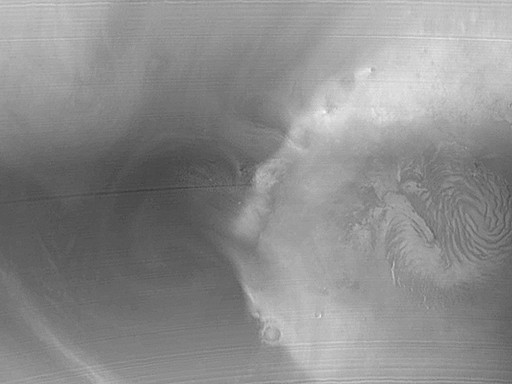
\includegraphics[scale=0.6]{images/Mars_surface.png}
	\end{figure}
	\vspace{-0.3cm}

	\paragraph{Procédé}	
		Pour remplir la mission nous avons calculé le taux de pixel, puis fais la somme des taux des pixels. Enfin, nous avons fait la moyenne du taux de gaz afin de déterminer la quantité de gaz dans l'atmosphère martienne. Nous n'avons pas eu besoin d'utiliser des filtres.
\clearpage
\subsection{Sous-mission A3}

	\begin{vwcol}[widths={0.65,0.2}, rule=0pt]
	\begin{minipage}{0.7\textwidth}
	\paragraph{Objectifs de la mission}

	Mettre en valeur les caneaux d'eau chaude sur une image en nuances de gris.
	\end{minipage}

	\begin{minipage}{0.25\textwidth}
	\begin{flushright}
	\paragraph{Technique utilisée}
	
	Seuillage
	\end{flushright}
	\end{minipage}

	\end{vwcol} 

	\begin{figure}[h]
	\centering
		\begin{multicols}{2}
		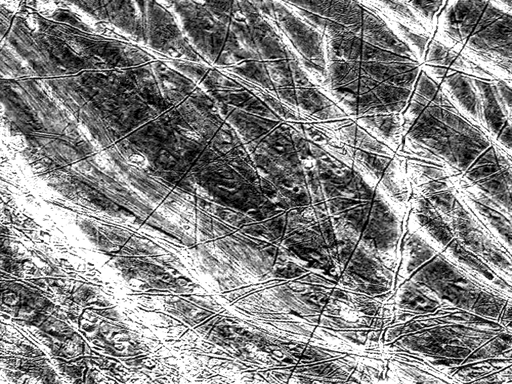
\includegraphics[scale=0.5]{images/Europa_surface.png}
		Avant

		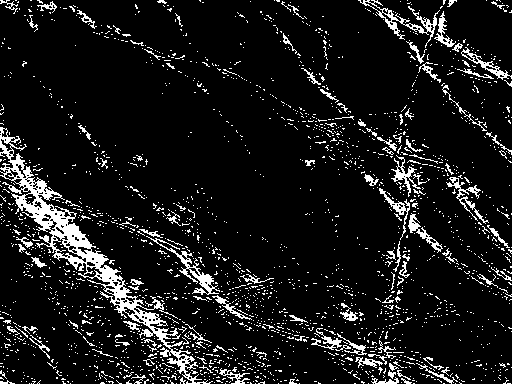
\includegraphics[scale=0.5]{images/MissionA3.png}
		Après
		\end{multicols}
	\end{figure}
	\vspace{-0.9cm}

	\paragraph{Procédé}	
		L'objectif de cette mission était de cartographier la circulation de l'eau sous la surface glacée de l'astre en ne faisant apparaître que les canaux d'eau chaude. Pour remplir la mission, nous avons utilisé un \emph{seuillage} afin d'observer les zones chaudes qui apparaissent en blanc.
\clearpage
	\subsection{Sous-mission A4}

	\begin{vwcol}[widths={0.65,0.2}, rule=0pt]
	\begin{minipage}{0.7\textwidth}
	\paragraph{Objectifs de la mission}

	Rendre une image de la planète Jupiter plus nette. Pour se faire nous avions à disposition deux photographies faites à quelques secondes d'intervalle comprenant toutes deux du bruit.
	\end{minipage}

	\begin{minipage}{0.3\textwidth}
	\begin{flushright}
	\paragraph{Techniques utilisés}

	Soustraction \& Filtre médian
	\end{flushright}
	\end{minipage}

	\end{vwcol} 

	\begin{figure}[h]
	\centering
		\begin{multicols}{2}
		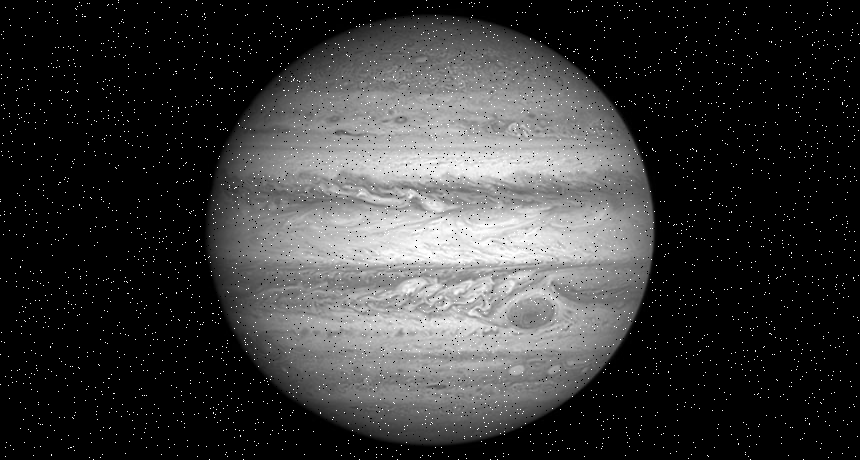
\includegraphics[scale=0.325]{images/Jupiter.png}
		Avant
		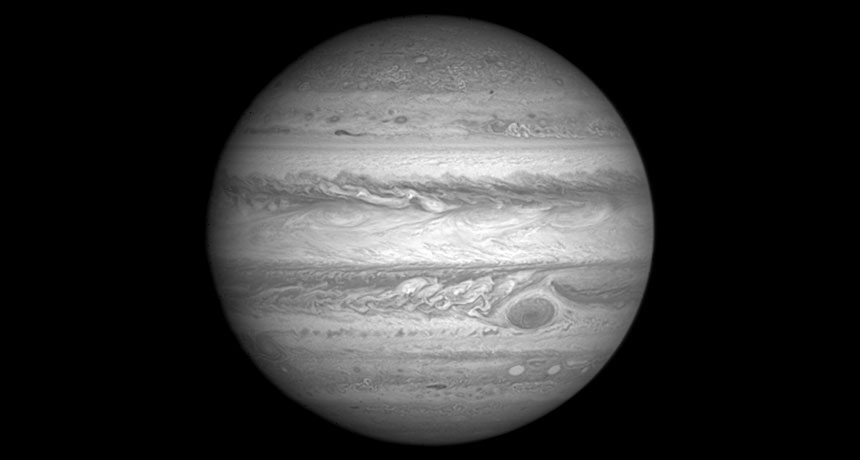
\includegraphics[scale=0.325]{images/JupiterAp.png}
		Après
		\end{multicols}
	\end{figure}
	\vspace{-0.9cm}

	\paragraph{Procédé}	
		Pour obtenir le résultat ci-dessus, nous avons utilisé deux filtres à la suite. Tout d'abord, nous avons \emph{soustrait} les deux images ensemble pour obtenir une troisième image ne comprenant que le bruit. Nous avons alors \emph{soustrait} ce résultat à l'image d'origine. Nous obtenons ensuite une image de meilleure qualité mais tout de même bruitée. Pour résoudre ce problème nous avons utilisé un \emph{filtre médian} permettant de retirer le bruit sans altérer la netteté de l'image.
\clearpage
\section{Mission B}
	\subsection{Sous-mission B1}

	\begin{vwcol}[widths={0.8,0.2}, rule=0pt]
	\begin{minipage}{0.7\textwidth}
	\paragraph{Objectifs de la mission}

	L'objectif de cette mission était de travailler l'image de Gliese 667Cc afin de faire apparaître son atmosphère sur les images prises par une sonde, cette image étant de mauvaise qualité. 
	\end{minipage}
	\begin{minipage}{0.2\textwidth}
		\begin{flushright}
			\paragraph{Filtre utilisé}
		Egalisation\up{\ref{Egalisation}}
		\end{flushright}
	\end{minipage}
	\end{vwcol} 

	\begin{figure}[h]
	\centering
		\begin{multicols}{2}
		
\includegraphics[scale=0.525]{images/Gliese667Cc.png}
		Avant
		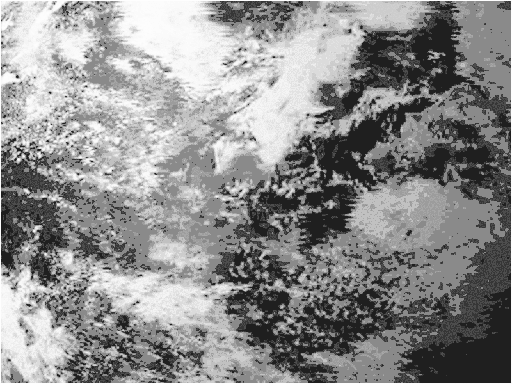
\includegraphics[scale=0.525]{images/Gliese667CcAFTER.png}
		Après
		\end{multicols}
	\end{figure}
	\vspace{-0.9cm}

		\paragraph{Procédé}	
			Pour cette mission une \emph{égalisation} a été réalisée sur cette image. Cette méthode fait nettement apparaître l'atmosphère de la planète. Une \emph{normalisation} avait été réalisée en premier lieu, qui faisait aussi apparaître cette atmosphère mais moins nettement.
\clearpage
\subsection{Sous-mission B2} 

	\begin{vwcol}[widths={0.8,0.2}, rule=0pt]
	\begin{minipage}{0.7\textwidth}
	\paragraph{Objectifs de la mission}

	L'objectif de cette mission était d'améliorer la visibilité de l'image afin de la donner à un autre service pour identifier la position d'une naine blanche située à 150 années lumière de la Terre.
	\end{minipage}
	\begin{minipage}{0.2\textwidth}
		\begin{flushright}
			\paragraph{Filtre utilisé}

			Normalisation\up{\ref{Normalisation}}
		\end{flushright}
	\end{minipage}
	\end{vwcol} 

	\begin{figure}[h]
	\centering
		\begin{multicols}{2}
		
\includegraphics[scale=0.525]{images/GD61.png}
		Avant
		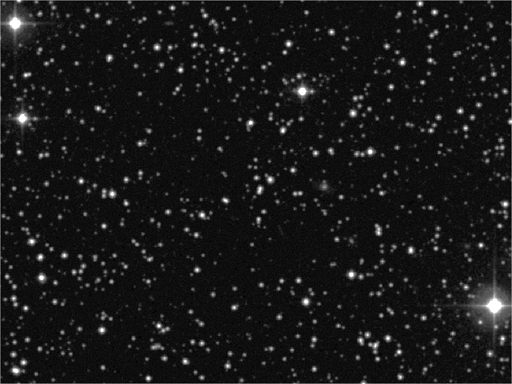
\includegraphics[scale=0.525]{images/GD61AFTER.png}
		Après
		\end{multicols}
	\end{figure}
	\vspace{-0.9cm}

		\paragraph{Procédé}	
			Pour cette mission une normalisation a été réalisée, faisant clairement apparaître les différentes planètes et étoiles.
\clearpage
\subsection{Sous-mission B3}
\clearpage
\section{Mission X}
	\subsection{Sous-mission X1}

	\begin{vwcol}[widths={0.8,0.2}, rule=0pt]
	\begin{minipage}{0.7\textwidth}
	\paragraph{Objectifs de la mission}

	Transformer l'image reçue par la sonde, pour savoir ce qui est arrivé à la sonde qui ne répond plus. Une image ressemblant à la transformée de Fourier de l'image originale a pu être récupérée.
	\end{minipage}
	\begin{minipage}{0.2\textwidth}
		\begin{flushright}
			\paragraph{Filtre utilisé}
		Transformée de Fourier inverse
		\end{flushright}
	\end{minipage}
	\end{vwcol} 

	\begin{figure}[h]
	\centering
		\begin{multicols}{2}
		
\includegraphics[scale=0.525]{images/X1.png}
		Avant
		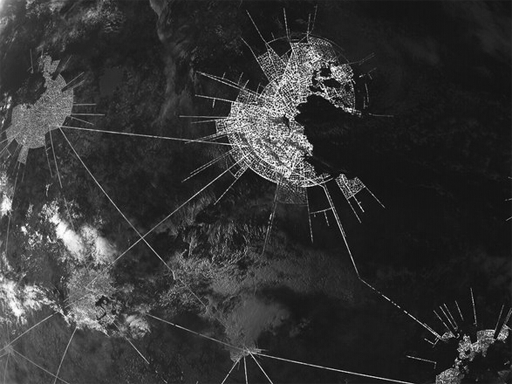
\includegraphics[scale=0.525]{images/X1AFTER.png}
		Après
		\end{multicols}
	\end{figure}
	\vspace{-0.9cm}

		\paragraph{Procédé}	
			Pour cette mission \emph{transformée de Fourier inverse} afin de retrouver l'image d'origine. La fonction native de Scilab \texttt{ifft} a été utilisée afin de faire l'opération inverse de transformation de Fourier. La fonction native a été utilisée pour sa rapidité et sa fiabilité.
\clearpage
\subsection{Sous-mission X2}

	\begin{vwcol}[widths={0.65,0.2}, rule=0pt]
	\begin{minipage}{0.7\textwidth}
	\paragraph{Objectifs de la mission}

	vérifier que ce qui apparaît sur l'image est bien de la végétation. L'image données est très perturbée par un bruit. Nous devons alors améliorer la visibilité en réduisant ce bruit.
	\end{minipage}

	\begin{minipage}{0.25\textwidth}
	\begin{flushright}
	\paragraph{Technique utilisée}
	
	Filtre median
	\end{flushright}
	\end{minipage}

	\end{vwcol} 

	\begin{figure}[h]
	\centering
		\begin{multicols}{2}
		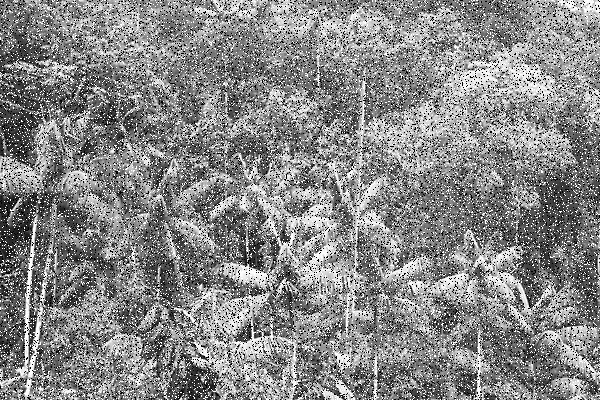
\includegraphics[scale=0.45]{images/Gliese_581d-V2.png}
		Avant

		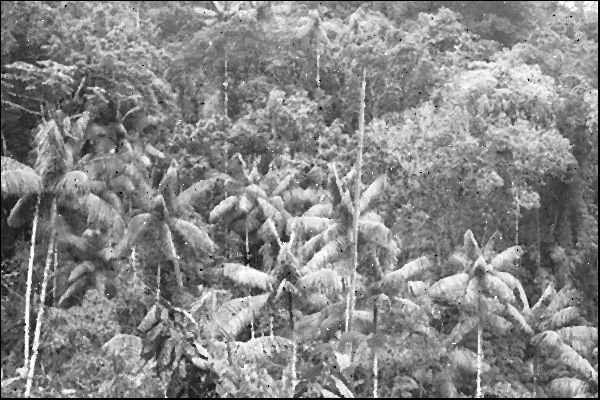
\includegraphics[scale=0.45]{images/MissionX2v2.png}
		Après
		\end{multicols}
	\end{figure}
	\vspace{-0.9cm}

	\paragraph{Procédé}
	
		Afin d'accomplir cette mission, il nous fallait nettoyer le bruit de l'image. Il était possible d'utiliser le filtre moyenneur et ou le filtre gaussien, mais le filtre médian surpasse ces deux filtres cités ci-dessus en terme de suppression de bruit et de qualité. Le filtre médian, permet de remplacer la valeur du pixel par la valeur médiane de son voisinage.
\clearpage
\subsection{Sous-mission U1}
\clearpage
\subsection{Sous-mission U2}

	\begin{vwcol}[widths={0.65,0.2}, rule=0pt]
	\begin{minipage}{0.7\textwidth}
	\paragraph{Objectifs de la mission}

	Mettre en valeur l'objet inconnu aparaissant sur l'image.
	\end{minipage}

	\begin{minipage}{0.3\textwidth}
	\begin{flushright}
	\paragraph{Techniques utilisés}

	Normalisation \& Detection des contours \& Isolation colorimétrique
	\end{flushright}
	\end{minipage}

	\end{vwcol} 

	\begin{figure}[h]
	\centering
		\begin{multicols}{2}
		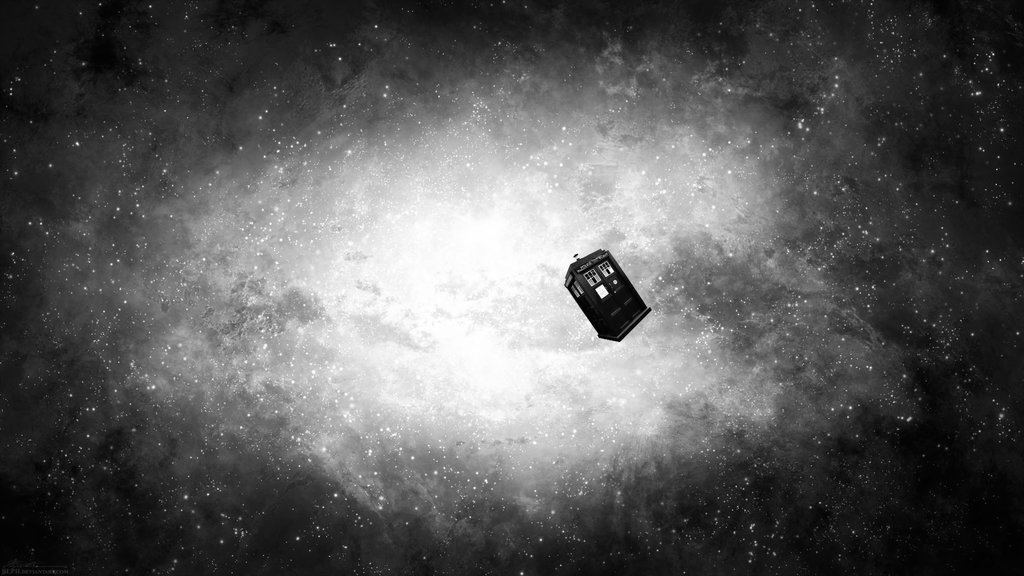
\includegraphics[scale=0.27]{images/U2_surface.png}
		Avant
		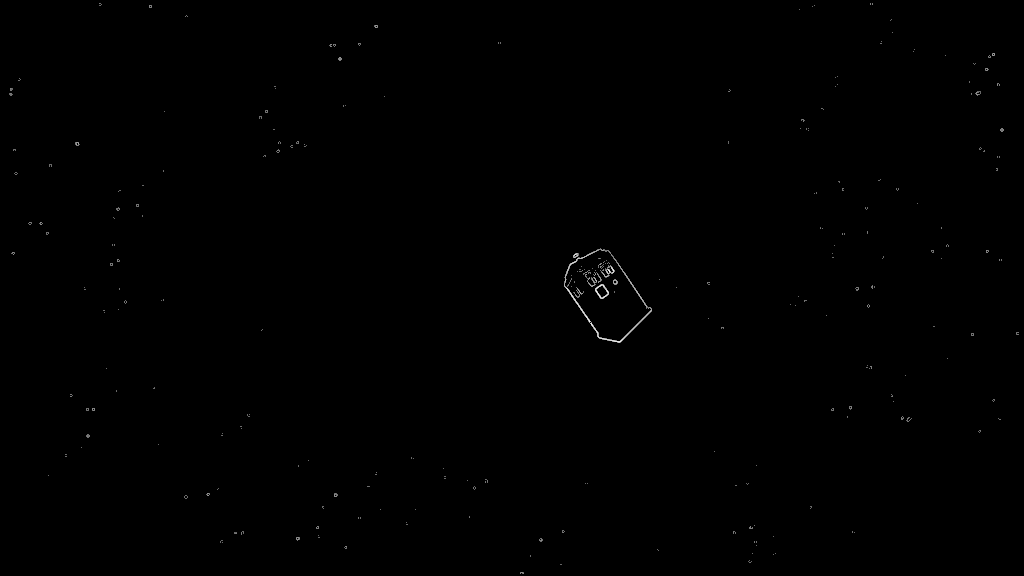
\includegraphics[scale=0.27]{images/MissionU2.png}
		Après
		\end{multicols}
	\end{figure}
	\vspace{-0.9cm}

	\paragraph{Procédé}	
		Pour mettre en valeur l'objet de l'image, nous avons tout d'abort éfféctué une \emph{detection de contour} sur l'image originale. Il en resulte le contour de l'OVNI. On éfféctue alors une \emph{normalisation} pour augmenter le contraste de l'image. Puis on séléctionne uniquement les couleurs les plus intenses pour retirer les pixels superflus.
\clearpage
\section{Filtres}
	
	\paragraph{Normalisation}
	\label{Normalisation}
	La normalisation est une méthode qui s'applique sur l'histogramme de l'image, afin d'effectuer une transformation affine du niveau de gris des pixels afin que l'image utilise toute la dynamique de représentation, dans notre cas avec des images 8 bits, la dynamique est étiré de 0 à 256 valeurs.


	\paragraph{Egalisation}

	\label{Egalisation}
	Cette méthode consiste à appliquer une transformation sur chaque pixel de l'image. Elle consiste en un ajustement du contraste de l'image qui utilise l'histogramme cumulé afin de chercher à obtenir un histogramme plat. Il a donc fallut construire un histogramme de l'image, puis normalisé cet histogramme. A partir de cet histogramme normalisé on peut construire un histogramme cumulé. A partir de cette histogramme cumulé, on peut enfin calculer chaque pixels de la nouvelle image.

	
	\paragraph{Seuillage}
	\label{Seuillage}

	Le seuillage est une méthode de segmentation d'image, à partir d'une image en niveau de gris, le seuillage d'image va créer une image binaire, comportant uniquement deux valeurs noir ou blanc. Par exemple si un seuil est défini à 120 alors la méthode va remplacer chaque pixel qui a une valeur supérieur à 120 par un pixel qui prendra la valeur 255  (blanc) et si la valeur est inférieur à 120 aors il prendra la valeur 0 (noir).

	\paragraph{Median}
	\label{Median}

	C'est un filtre utilisé pour réduire le bruit d'une image. Le principe du filtre est de remplacer chaque pixel par la valeur médiane de son voisinage. Il va considérer les valeurs du voisinage par valeurs croissantes et prendre la valeur médiane, ce qui permet de remplacer des valeurs dites abberantes par une valeur de consensus entre les valeurs voisines. Ce filtre à l'avantage de respecter les contours et le contraste de l'image.

	\paragraph{Convolution}

	\label{Convolution}


	\paragraph{Fourier}
	\label{Fourier}


	La convolution est l'opérateur de base du traitement linéaire des images. Pour calculer une convolution, on remplace la valeur de chaque pixel par la valeur du produit scalaire entre les valeurs du voisinage du pixel considéré.
	


\clearpage

\section{Algorithmes de traitement}

Par besoin de conscision, nous n'avons pas inclus le code de nos algorithmes dans le raport. En revanche, l'ensemble de nos filtres sont disponibles dans notre dossier \texttt{scripts} sur GitHub (\href{https://github.com/Exia-epickiwi/exolife/tree/master/scripts}{\texttt{goo.gl/yA9lvK}}).

L'ensemble des programmes de mission sont aussi disponibles dans le dossier \texttt{workspace} sur GitHub (\href{https://github.com/Exia-epickiwi/exolife/tree/master/workspace}{\texttt{goo.gl/DBfesI}}).

Pour des informations générales sur le projet et tout les fichiers qui lui sont attachés, vous pouvez consulter le dépot général GitHub (\href{https://github.com/Exia-epickiwi/exolife}{\texttt{goo.gl/KPSNnZ}}), vous y trouverez les mission, les images, les algorithmes de filtrage et le code source du rapport.

\section{Bilan personnels}

\paragraph{\bsc{Saclier} Baptiste} Ce projet fut une très bonne experience dans le domaine des mathématiques et une très bonne introduction à l'imagerie, un domaine très intéressant et en plein essor actuellement. Ce fut un bon retour aux sciences avec un bon sujet.

Durant le projet, l'ensemble du groupe était motivé et une bonne utilisation d'outils comme GitHub et Slack ont permis une très bonne cohésion et une bonne communication entre les membres.

\paragraph{\bsc{Chiaverini} Marie}

Cela fut un projet rapide, travailler sur un autre sujet qui est l'imagerie est intéressant, connaître les différents aspects de filtre et méthode est assez enrichissant. Néanmoins, en fin de semaine, j'ai commencé à avoir une certaine lassitude, c'est un sujet auquel je travaillerai rarement. Le projet est assez bien, l'équipe aussi, ils ont été assez patient et m'ont bien aider lors de certaine mission.

\paragraph{\bsc{Blochet} Tanguy}

\section{Bilan général}
\vspace{-0.5cm}\hspace{0.5cm}\textit{du chef de projet Chiaverini Marie}
\vspace{0.5cm}

Il y a eu une bonne ambiance et une bonne entraide dans l'équipe. Nous avons pas eu de difficulté en ce qui concerne l'organisation. Les tâches ont été terminés à temps. Le travail effectué avec le groupe est satisfaisante.
\end{document}